\begin{ex}
 (Unesp) Dado um poliedro de 5 vértices e 6 faces triangulares, escolhem-se ao acaso três dos seus vértices.

% DEFINING COLORS COF, PUR, GREEO AND GREET
\definecolor{cof}{RGB}{219,144,71}
\definecolor{pur}{RGB}{186,146,162}
\definecolor{greeo}{RGB}{91,173,69}
\definecolor{greet}{RGB}{52,111,72}

\begin{center}
% Bi-pyramid
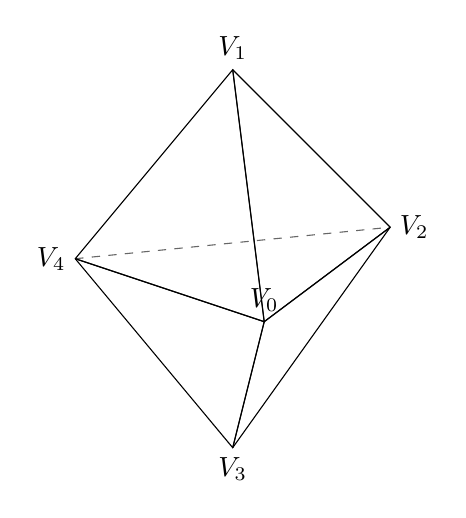
\begin{tikzpicture}[scale=4]
\coordinate [label=left:$V_4$] (V4) at (0,0);
\coordinate [label=right:$V_2$] (V2) at (1,0.1) ;
\coordinate [label=above:$V_0$] (V0) at (0.6,-0.2);
\coordinate [label=above:$V_1$] (V1) at (0.5,0.6) ;
\coordinate [label=below:$V_3$] (V3) at (0.5,-0.6);
%
\begin{scope}[dashed,,opacity=0.6]
\draw (V4)  -- (V2);
\end{scope}

\draw (V4) -- (V0) -- (V1) ;
\draw (V4) -- (V0) -- (V3);
\draw (V2) -- (V0) -- (V1);
\draw (V2) -- (V0) -- (V3);
%
\draw (V1) -- (V4) -- (V3) -- (V2) --cycle;
%
\end{tikzpicture}
\end{center}
A probabilidade de que os três vértices escolhidos pertençam à mesma face do poliedro é:
    \begin{enumerate}[(a)]
    \item $\frac{3}{10}$
    \item $\frac{1}{6}$
    \item $\frac{3}{5}$
    \item $\frac{1}{5}$
    \item $\frac{6}{35}$
    \end{enumerate}
      \begin{sol}
       resposta: c \\
       $p=\frac{6}{\mathrm{C}_{5,3}}=\frac{3}{5}$
      \end{sol}
\end{ex}